\question{}

คำถามเกี่ยวกับการลากเส้นรูปปิดตามโครงสร้างที่กำหนดให้

\smallskip\noindent
\textbf{\uline{ตัวอย่าง}}\; จากรูปที่แสดงทาง\ifpageodd{ขวา}{ซ้าย}มือนี้
\marginnote{%
    \centering
    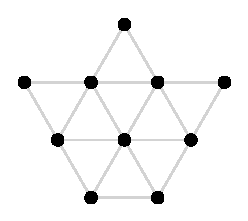
\includegraphics{figures/quickfire_central_regional_closedshapearea_01.eps}
}
มีโครงสร้างเรขาคณิตที่เรียงตัวเป็นสามเหลี่ยมด้านเท่าย่อย ๆ หลายรูปประกอบกัน
โดยที่สามเหลี่ยมย่อยแต่ละรูปมีพื้นที่รูปละ 1 ตารางหน่วย

จากโครงสร้างเรขาคณิตรูปนี้ เราจะพยายามลากเส้นภายในโครงสร้างที่กำหนดให้ข้างต้น โดยมีเงื่อนไขว่า
\begin{itemize}
\item เราจะต้องลากเส้นเพียงเส้นเดียว ผ่านจุดยอดให้ครบทุกจุด แล้วกลับมายังจุดเริ่มต้น กลายเป็นรูปปิด
\item จุดยอดแต่ละจุดจะต้องถูกเยือน 1 ครั้งพอดี ไม่ขาดและไม่เกิน
\item เส้นทุกเส้นที่ลากผ่านจะต้องมีเค้าโครงเดิมจากเส้นสีเทาที่กำหนดให้จากรูปดั้งเดิม
\item รูปปิดที่เกิดขึ้นจะต้องมี\uline{พื้นที่ภายในมากที่สุด}เท่าที่เป็นไปได้
\end{itemize}

\marginnote{%
    \centering
    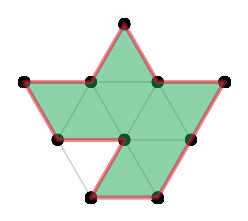
\includegraphics{figures/quickfire_central_regional_closedshapearea_02.eps}
}

รูปที่สองที่ปรากฏทางด้าน\ifpageodd{ขวา}{ซ้าย}มือนี้
แสดงหนึ่งในวิธีที่เราสามารถลากเส้นรูปปิดภายในโครงสร้างเรขาคณิต (ดังที่แสดงในรูปแรก)
ที่สอดคล้องกับเงื่อนไขที่กล่าวมาข้างต้นได้ทั้งหมด ซึ่งรูปปิดดังกล่าวจะได้พื้นที่ภายในรวม 8 ตารางหน่วย\;
(\textbf{หมายเหตุ:} อาจมีวิธีลากเส้นวิธีอื่น~ๆ ที่ทำให้ได้พื้นที่ขนาดเท่ากัน)

\medskip\noindent
\textbf{\uline{โจทย์}}\; 
จงหาว่าในรูปต่อไปนี้ เราจะลากเส้นสร้างรูปปิดตามเงื่อนไขเดียวกันให้ได้พื้นที่ภายในมากที่สุด จะได้พื้นที่เท่าใด?
\begin{center}
    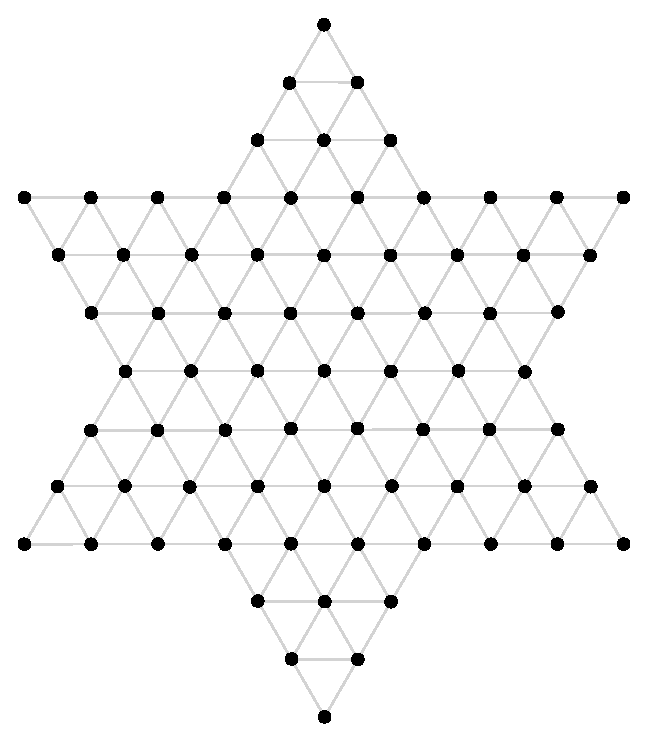
\includegraphics[width=0.7\linewidth]{figures/quickfire_central_regional_closedshapearea_03.eps}
\end{center}